% Requires graphicx; uses the existing AnchorFathomGPT bibliography entry.
% Place fathomgpt_observer_map.png in figures/.
% Publication reuse permission remains unconfirmed; see README.md.
\begin{figure}[t]
  \centering
  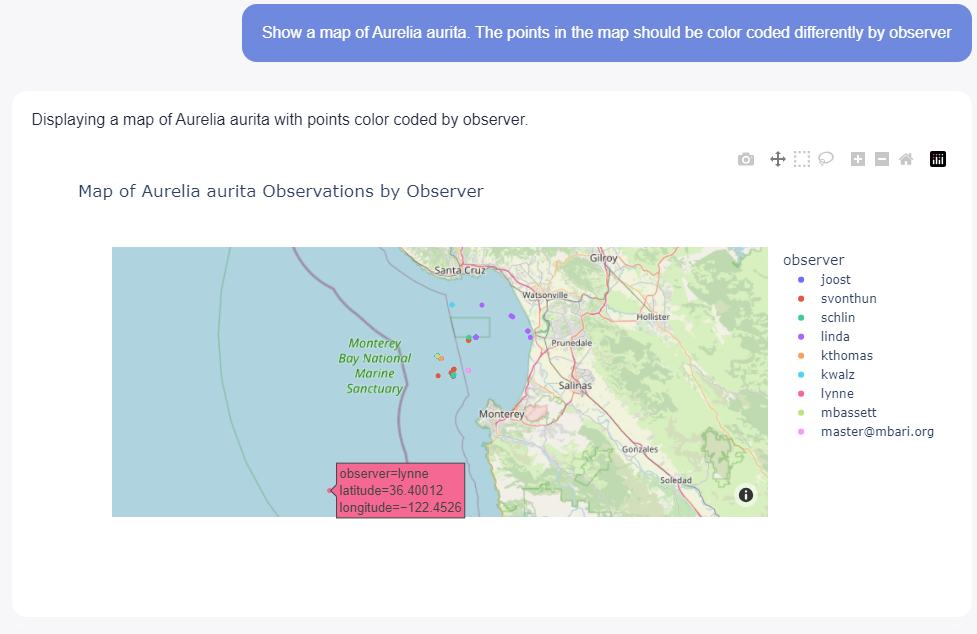
\includegraphics[width=\linewidth]{figures/system-examples/fathomgpt_observer_map.png}
  \caption{FathomGPT translates a natural-language request into an interactive map of \textit{Aurelia aurita} observations, with points colored by observer. The scientist specifies the species and grouping, while the system constructs the visualization; hovering reveals the observer and coordinates of an individual record. This connects Conversational assistance to spatial comparison and inspection of observation metadata on a Desktop/Planar display. Source: Khanal et al.~\cite{AnchorFathomGPT}, Fig.~12. Copyright 2024 held by the owner/author(s).}
  \label{fig:fathomgpt-observer-map}
\end{figure}
